%%%%%%%%%%%%%%%%%%%%%%%%%%%%%%%%%%%%%%%%%%%%%%%%%%%%%%%%%%%%%%%%%%%%%%%%%%%%%%%%%%%%%%%%%
\frame[t]
{
	\frametitle{Story of computing}
	\framesubtitle{The Beginning}
   	\begin{itemize}
		\item 	During World War II, Alan Turing - a British mathematician started to work
		with Britain's code-breaking centre and deciphered Germany's U-boat Enigma, saving 
		battle of the Atlantic! 
	  	\item	He conceived the principles of modern computers and brought about
	  	his famous "Turing's Machine" in 1936. 
	  	\item "Turing's Machine" is a hypothetical device that manipulates symbols 
	  	on a strip of tape according to a table of rules which could simulate the logic of
	  	almost any computer algorithm.
   	\end{itemize}	

   	  
	\end{block}
}
%%%%%%%%%%%%%%%%%%%%%%%%%%%%%%%%%%%%%%%%%%%%%%%%%%%%%%%%%%%%%%%%%%%%%%%%%%%%%%%%%%%%%%%%%


%%%%%%%%%%%%%%%%%%%%%%%%%%%%%%%%%%%%%%%%%%%%%%%%%%%%%%%%%%%%%%%%%%%%%%%%%%%%%%%%%%%%%%%%%
\frame[t]
{
	\frametitle{Story of computing continues}
	\framesubtitle{The Beginning}
   		\begin{itemize}
			\item On the other side of the spectrum Konrad Zuse - 
			a German civil engineer in Berlin - started dreaming of a machine that could do 
			mechanical calculations.
			\item He started working in his parents' apartment and built his 
			first electro-mechanical computer – Z1 in the same year 1936.
			\item It was a floating point binary mechanical calculator with limited 
			programmability, reading instructions from a perforated 35 mm film.
		\end{itemize}
		
		So we had a rare situation of two people coming from two different 
		backgrounds and laying foundations for the modern day computing and computer science.
	\end{block}
}
%%%%%%%%%%%%%%%%%%%%%%%%%%%%%%%%%%%%%%%%%%%%%%%%%%%%%%%%%%%%%%%%%%%%%%%%%%%%%%%%%%%%%%%%%


%%%%%%%%%%%%%%%%%%%%%%%%%%%%%%%%%%%%%%%%%%%%%%%%%%%%%%%%%%%%%%%%%%%%%%%%%%%%%%%%%%%%%%%%%
\frame[t]
{
  \frametitle{Frame Title}
      \begin{block}{Block Title}
   \begin{itemize}%[<+-| alert@+>]
	\item One
	\item Two

   \begin{itemize}
   	\item One.one
	\item One.two
   \end{itemize}
	\item More information at \\ {\footnotesize \url{https://http://www.cray.com/About/History.aspx}}.
   \end{itemize}
  \end{block}
}
%%%%%%%%%%%%%%%%%%%%%%%%%%%%%%%%%%%%%%%%%%%%%%%%%%%%%%%%%%%%%%%%%%%%%%%%%%%%%%%%%%%%%%%%%


%%%%%%%%%%%%%%%%%%%%%%%%%%%%%%%%%%%%%%%%%%%%%%%%%%%%%%%%%%%%%%%%%%%%%%%%%%%%%%%%%%%%%%%%%
\frame[t]
{
  \frametitle{First computers}
      \begin{block}{Monolithic}
   \begin{itemize}
	\item One
	\item Two

   \begin{itemize}
   	\item One.one
	\item One.two
   \end{itemize}
	\item More information at \\ {\footnotesize \url{https://www.domain.org.nz}}.
   \end{itemize}
  \end{block}
}
%%%%%%%%%%%%%%%%%%%%%%%%%%%%%%%%%%%%%%%%%%%%%%%%%%%%%%%%%%%%%%%%%%%%%%%%%%%%%%%%%%%%%%%%%


%%%%%%%%%%%%%%%%%%%%%%%%%%%%%%%%%%%%%%%%%%%%%%%%%%%%%%%%%%%%%%%%%%%%%%%%%%%%%%%%%%%%%%%%%%
\frame[t]
{
  \frametitle{Story of computing}
    \framesubtitle{Need for speed}
      \begin{block}{Cray vs Grandma's PC!}
            \begin{center}
       \begin{small}
      \begin{tabular}{|l|l|l|}
      \hline 
      \textbf{Feature/System} & \textbf{Cray 2} & \textbf{Grandma's PC} \\ 
      \hline 
      MegaFlops & 1000 (1 GFlops) & \$32 Million (Inflation adjusted) \\ 
      \hline 
      Cost & 25000 (25GFlops) & \$600  \\ 
      \hline 
      \end{tabular} 
      \end{small}
      \end{center}    
       
  	Apollo 11, the spaceflight that took Neil Armstrong and Buzz Aldrin to moon was 
 	powered by Apollo Guidance Computer (AGC), which is less powerful than most 
 	our smartphones! 
  	\end{block}
  
    %\begin{center}
  		%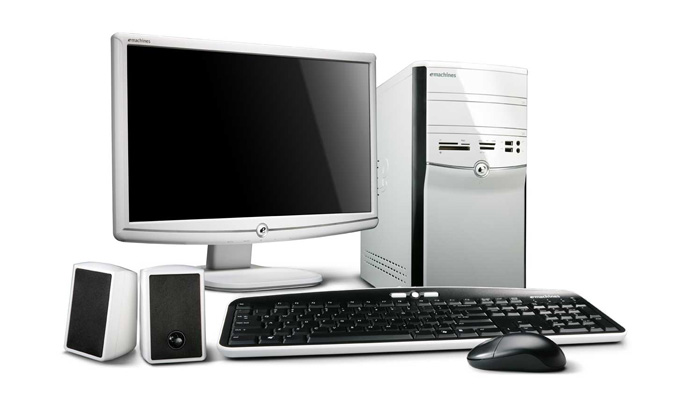
\includegraphics[width=100pt]{fig/pc.jpg}
 	%\end{center}
 	

 	
}
%%%%%%%%%%%%%%%%%%%%%%%%%%%%%%%%%%%%%%%%%%%%%%%%%%%%%%%%%%%%%%%%%%%%%%%%%%%%%%%%%%%%%%%%%%

%%%%%%%%%%%%%%%%%%%%%%%%%%%%%%%%%%%%%%%%%%%%%%%%%%%%%%%%%%%%%%%%%%%%%%%%%%%%%%%%%%%%%%%%%
\frame[t]
{
  \frametitle{Story of computing}
      \framesubtitle{Need for speed}
    	Just a side story: what do we do with that kind of computing power, now?	
   		\begin{center}
 			\includegraphics[width=200pt]{fig/angry-birds-phone.jpg}
   		\end{center}
   		
   		\begin{itemize}
			\item	It just shows our insatiable need for speed and computing power!
			\item	History took a turn in its course.
		\end{itemize}
}
%%%%%%%%%%%%%%%%%%%%%%%%%%%%%%%%%%%%%%%%%%%%%%%%%%%%%%%%%%%%%%%%%%%%%%%%%%%%%%%%%%%%%%%%%



%%%%%%%%%%%%%%%%%%%%%%%%%%%%%%%%%%%%%%%%%%%%%%%%%%%%%%%%%%%%%%%%%%%%%%%%%%%%%%%%%%%%%%%%%%

\frame[t]
{
  \frametitle{Hegelian dialectics}
      \framesubtitle{Two rules that went wrong!}
      \begin{block}{Rules go wrong}
      Physicist Michio Kaku, a professor of theoretical physics at City University 
      of New York, said in a videotaped interview on BigThink.com that time is running 
      out on the 47-year-old law. 
      "In about 10 years or so, we will see the collapse 
      of Moore's Law," 
      
      two main problems that will derail Moore's Law are heat and leakage where the age
      of silicon will be over.
      
      
      It’s the first time [we've had these troubles] in quite a number of generations,
      ' Intel's William Holt told the Wall Street Journal at the invitation-only 
      investor's day. 'It’s just getting really hard. [The problem is] just getting 
      the size down. As hard as it is, it’s going to be just as hard for everybody else,
      ' Holt added, reassuring investors that the problems aren't exclusive to the company.
      
      There's a lower limit to how many times the process node can shrink
      
      Traditionally, it's been that doubling in performance that has kept its customers 
      upgrading year after year - and each process node shrink comes with a corresponding 
      decrease in base manufacturing costs which helps offset the research and development 
      needed in order to reach a given node.
      
  \end{block}
}

%%%%%%%%%%%%%%%%%%%%%%%%%%%%%%%%%%%%%%%%%%%%%%%%%%%%%%%%%%%%%%%%%%%%%%%%%%%%%%%%%%%%%%%%%%

\begin{frame}[fragile]
  \frametitle{Title}
      \begin{block}{Sub Title}

      \end{block}
\end{frame}

%%%%%%%%%%%%%%%%%%%%%%%%%%%%%%%%%%%%%%%%%%%%%%%%%%%%%%%%%%%%%%%%%%%%%%%%%%%%%%%%%%%%%%%%%%
%%%%%%%%%%%%%%%%%%%%%%%%%%%%%%%%%%%%%%%%%%%%%%%%%%%%%%%%%%%%%%%%%%%%%%%%%%%%%%%%%%%%%%%%%%
\begin{frame}[fragile,shrink]
  \frametitle{Title}
      \begin{block}{Sub Title}

  \end{block}
\end{frame}

%%%%%%%%%%%%%%%%%%%%%%%%%%%%%%%%%%%%%%%%%%%%%%%%%%%%%%%%%%%%%%%%%%%%%%%%%%%%%%%%%%%%%%%%%%

\begin{frame}[fragile]
\begin{algorithm}[H]
\begin{algorithmic}[1]
\FOR{$i=1$ to $N$}
\FOR{$j=1$ to $JJJJ$}
\STATE $energy[i*JJJ+j] =$ \\
$ interpolate(AAA[i*JJJ+j], ZZZ)$
\ENDFOR
\ENDFOR
\end{algorithmic}
\caption{pseudocode for the calculation of }
\label{alg:seq}
\end{algorithm}
\end{frame}

%%%%%%%%%%%%%%%%%%%%%%%%%%%%%%%%%%%%%%%%%%%%%%%%%%%%%%%%%%%%%%%%%%%%%%%%%%%%%%%%%%%%%%%%%%
\frame[t]
{
  \frametitle{Parallel problems}
      %\begin{block}{N body problem}
      	\begin{frame}[fragile]
		\begin{algorithm}[H]
		\begin{algorithmic}[1]


\FOR{$i=1$ to $N$}
\FOR{$j=1$ to $JJJJ$}
\STATE $energy[i*JJJ+j] =$ \\
$ interpolate(AAA[i*JJJ+j], ZZZ)$
\ENDFOR
\ENDFOR

\end{algorithmic}
\caption{pseudocode for N Body Problem}
\label{alg:seq}
\end{algorithm}
\end{frame}
   
  %\end{block}
}